%
% test file for building one chapter
%

\documentclass[12pt]{book}

\title{Think Java}
\author{Allen B. Downey and Chris Mayfield}

\newcommand{\thetitle}{Think Java}
\newcommand{\thesubtitle}{How to Think Like a Computer Scientist}
\newcommand{\theauthors}{Allen B. Downey and Chris Mayfield}
\newcommand{\theversion}{2nd Edition, Version 7.0.0 DRAFT}

%%%% Both LATEX and PLASTEX

\usepackage{graphicx}
\usepackage{setspace}

% automatically index glossary terms
\newcommand{\term}[1]{%
\item[#1:]\index{#1}}

\usepackage{amsmath}
\usepackage{amsthm}

% format end of chapter excercises
\newtheoremstyle{exercise}
  {12pt}        % space above
  {12pt}        % space below
  {}            % body font
  {}            % indent amount
  {\bfseries}   % head font
  {}            % punctuation
  {12pt}        % head space
  {}            % custom head
\theoremstyle{exercise}
\newtheorem{exercise}{Exercise}[chapter]

\newif\ifplastex
\plastexfalse

%%%% PLASTEX ONLY
\ifplastex

\makeindex

\usepackage{localdef}

\usepackage{url}
\renewcommand{\href}[2]{\url{#1}}

\makeatletter
\newcount\anchorcnt
\newcommand*{\Anchor}[1]{%
  \@bsphack%
    \Hy@GlobalStepCount\anchorcnt%
    \edef\@currentHref{anchor.\the\anchorcnt}%
    \Hy@raisedlink{\hyper@anchorstart{\@currentHref}\hyper@anchorend}%
    \M@gettitle{}\label{#1}%
    \@esphack%
}
\makeatother

% code listing environments:
% we don't need these for plastex because they get replaced
% by preprocess.py
%\newenvironment{code}{\begin{verbatim}}{\end{verbatim}}
%\newenvironment{stdout}{\begin{verbatim}}{\end{verbatim}}

% inline syntax formatting
\newcommand{\java}{\verb}%}
\newcommand{\textcolor}[1]{\relax}

%%%% LATEX/HTML ONLY
\else

%BEGIN LATEX
\usepackage{comment}
\excludecomment{htmlonly}
\includecomment{latexonly}
%END LATEX

\usepackage{geometry}
\geometry{
    width=5.5in,
    height=8.5in,
    hmarginratio=3:2,
    vmarginratio=1:1,
    includehead=true,
    headheight=15pt
}

% paragraph spacing
\setlength{\parindent}{0pt}                      % 17.62482pt
\setlength{\parskip}{12pt plus 4pt minus 4pt}    % 0.0pt plus 1.0pt
\linespread{1.05}
\def\arraystretch{1.5}

% list spacing
\setlength{\topsep}{5pt plus 2pt minus 3pt}      % 10.0pt plus 4.0pt minus 6.0pt
\setlength{\partopsep}{-6pt plus 2pt minus 2pt}  %  3.0pt plus 2.0pt minus 2.0pt
\setlength{\itemsep}{0pt}                        %  5.0pt plus 2.5pt minus 1.0pt

% these are copied from tex/latex/base/book.cls
% all I changed is afterskip
\makeatletter
\renewcommand{\section}{\@startsection{section}{1}{\z@}%
    {-3.5ex \@plus -1ex \@minus -.2ex}%
    {0.7ex \@plus.2ex}%
    {\normalfont\Large\bfseries}}
\renewcommand\subsection{\@startsection{subsection}{2}{\z@}%
    {-3.25ex\@plus -1ex \@minus -.2ex}%
    {0.3ex \@plus .2ex}%
    {\normalfont\large\bfseries}}
\renewcommand\subsubsection{\@startsection{subsubsection}{3}{\z@}%
    {-3.25ex\@plus -1ex \@minus -.2ex}%
    {0.3ex \@plus .2ex}%
    {\normalfont\normalsize\bfseries}}
\makeatother

% table of contents vertical spacing
\usepackage{tocloft}
\setlength\cftparskip{8pt plus 4pt minus 4pt}

% balanced index with TOC entry
\usepackage[totoc]{idxlayout}

% The following line adds a little extra space to the column
% in which the Section numbers appear in the table of contents
\makeatletter
\renewcommand{\l@section}{\@dottedtocline{1}{1.5em}{3.0em}}
\makeatother

% customize page headers
\usepackage{fancyhdr}
\pagestyle{fancyplain}
\renewcommand{\chaptermark}[1]{\markboth{Chapter \thechapter ~~ #1}{}}
\renewcommand{\sectionmark}[1]{\markright{\thesection ~~ #1}}
\lhead[\fancyplain{}{\bfseries\thepage}]%
      {\fancyplain{}{\bfseries\rightmark}}
\rhead[\fancyplain{}{\bfseries\leftmark}]%
      {\fancyplain{}{\bfseries\thepage}}
\cfoot{}
\usepackage[mmddyyyy]{datetime}
\rfoot{\textcolor{gray}{\tiny \thetitle, \theversion, \today}}

%% tweak spacing of figures and captions
%\usepackage{floatrow}
%\usepackage{caption}
%\captionsetup{
%    font=small,
%    labelformat=empty,
%    justification=centering,
%    skip=4pt
%}

% colors for code listings and output
\usepackage{xcolor}
\definecolor{bgcolor}{HTML}{FAFAFA}
\definecolor{comment}{HTML}{007C00}
\definecolor{keyword}{HTML}{0000FF}
\definecolor{strings}{HTML}{B20000}

% syntax highlighting in code listings
\usepackage{textcomp}
\usepackage{listings}
\lstset{
    language=java,
    basicstyle=\ttfamily,
    backgroundcolor=\color{bgcolor},
    commentstyle=\color{comment},
    keywordstyle=\color{keyword},
    stringstyle=\color{strings},
    columns=fullflexible,
    emph={label},  % keyword?
    keepspaces=true,
    showstringspaces=false,
    upquote=true,
    xleftmargin=15pt,  % \parindent
    framexleftmargin=3pt,
    aboveskip=\parskip,
    belowskip=\parskip
}

% code listing environments
\lstnewenvironment{code}
{\minipage{\linewidth}}
{\endminipage}
\lstnewenvironment{stdout}
{\lstset{commentstyle=,keywordstyle=,stringstyle=}\minipage{\linewidth}}
{\endminipage}

% interactive code listing
\lstnewenvironment{trinket}[2][400]
{\minipage{\linewidth}}
{\endminipage}

% inline syntax formatting
\newcommand{\java}[1]{\lstinline{#1}}%{

% prevent hyphens in names
\hyphenation{DrJava}
\hyphenation{GitHub}
\hyphenation{Javadoc}

% pdf hyperlinks, table of contents, and document properties
\usepackage{hyperref}
\hypersetup{%
  pdftitle={\thetitle: \thesubtitle},
  pdfauthor={\theauthors},
  pdfsubject={Version \theversion},
  pdfkeywords={},
  bookmarksopen=false,
  bookmarksnumbered=true,
  colorlinks=true,
  citecolor=black,
  filecolor=black,
  linkcolor=black,
  urlcolor=blue
}

% add dot after numbers in pdf bookmarks
\makeatletter
\renewcommand{\Hy@numberline}[1]{#1. }
\makeatother


\fi

%%%% END OF PREAMBLE
\begin{document}

\setcounter{chapter}{15}
\setcounter{page}{0}

\tableofcontents

\chapter{Reusing Classes}

In Chapter~\ref{conway}, we developed classes to implement Conway's Game of Life.
%As an exercise, you had a chance to implement Langton's Ant.
We can reuse the \java{Cell} and \java{GridCanvas} classes to implement other simulations.
One of the most interesting zero-player games is {\it Langton's Ant}, which models an ``ant'' that walks around a grid.
The ant follows only two simple rules:

\begin{enumerate}
\item If the ant is on a white cell, it turns to the right, makes the cell black, and moves forward.
\item If the ant is on a black cell, it turns to the left, makes the cell white, and moves forward.
\end{enumerate}

Because the rules are simple, you might expect the ant to do something simple, like make a square or repeat a simple pattern.
But starting on a grid with all white cells, the ant makes more than 10,000 steps in a seemingly random pattern before it settles into a repeating loop of 104 steps.
You can read more about it at \url{https://en.wikipedia.org/wiki/Langton's_ant}.

%Reusing the classes we developed in this chapter, write an implementation of Langton's Ant.
%We present a solution to this exercise in Appendix~\ref{app:langton}.

In this chapter, we present a solution to Langton's Ant and use it to demonstrate more advanced object-oriented techniques.


\section{Langton's Ant}

We begin by defining a \java{Langton} class that has a grid and information about the ant.
The constructor takes the grid dimensions as parameters.

\begin{code}
public class Langton {
    private GridCanvas grid;
    private int xpos;
    private int ypos;
    private int head; // 0=North, 1=East, 2=South, 3=West

    public Langton(int rows, int cols) {
        grid = new GridCanvas(rows, cols, 10);
        xpos = rows / 2;
        ypos = cols / 2;
        head = 0;
    }
}
\end{code}

\java{grid} is a \java{GridCanvas} object, which represents the state of the cells.
\java{xpos} and \java{ypos} are the coordinates of the ant, and \java{head} is the ``heading'' of the ant, that is, what direction it is facing.
\java{head} is an integer with four possible values, where 0 means the ant is facing ``north'', that is, toward the top of the screen, 1 means ``east'', etc.

Here's an \java{update} method that implements the rules for Langton's ant:

\begin{code}
public void update() {
    flipCell();
    moveAnt();
}
\end{code}

The \java{flipCell} method gets the \java{Cell} at the ant's location, figures out which way to turn, and changes the state of the cell.

\begin{code}
private void flipCell() {
    Cell cell = grid.getCell(xpos, ypos);
    if (cell.isOff()) {
        head = (head + 1) % 4;    // turn right
        cell.turnOn();
    } else {
        head = (head + 3) % 4;    // turn left
        cell.turnOff();
    }
}
\end{code}

We use the remainder operator, \verb"%", to make \java{head} wrap around: if \java{head} is 3 and we turn right, it wraps around to 0; if \java{head} is 0 and we turn left, it wraps around to 3.

Notice that to turn right, we add 1 to \java{head}.
To turn left, we could subtract 1, but \verb"-1 % 4" is \verb"-1" in Java.
So we add 3 instead, since one left turn is the same as three right turns.

The \java{moveAnt} method moves the ant forward one square, using \java{head} to determine which way is forward.

\begin{code}
private void moveAnt() {
    if (head == 0) {
        ypos -= 1;
    } else if (head == 1) {
        xpos += 1;
    } else if (head == 2) {
        ypos += 1;
    } else {
        xpos -= 1;
    }
}
\end{code}

Here is the \java{main} method we use to create and display the \java{Langton} object:

\begin{code}
public static void main(String[] args) {
    String title = "Langton's Ant";
    Langton game = new Langton(61, 61);
    JFrame frame = new JFrame(title);
    frame.setDefaultCloseOperation(JFrame.EXIT_ON_CLOSE);
    frame.setResizable(false);
    frame.add(game.grid);
    frame.pack();
    frame.setVisible(true);
    game.mainloop();
}
\end{code}

Most of this code is the same as the \java{main} we used to create and run \java{Conway}, in Section~\ref{conwaymain}.
It creates and configures a \java{JFrame} and runs \java{mainloop}.

And that's everything!
If you run this code with a grid size of \mbox{61 x 61} or larger, you will see the ant eventually settle into a repeating pattern.

Because we designed \java{Cell} and \java{GridCanvas} to be reusable, we didn't have to modify them at all.
However, we now have two copies of the \java{main} method---one on \java{Conway}, and one in \java{Langton}.


\section{Refactoring}

Whenever you see repeated code like \java{main}, you should think about ways to remove it.
In the Chapter~\ref{eights}, we used inheritance to eliminate repeated code.
We'll do something similar with \java{Conway} and \java{Langton}.

First, we define a superclass named \java{Automaton} where we will put the code that \java{Conway} and \java{Langton} have in common.

\begin{code}
public class Automaton {
    private GridCanvas grid;

    public void run(String title, int rate) {
        JFrame frame = new JFrame(title);
        frame.setDefaultCloseOperation(JFrame.EXIT_ON_CLOSE);
        frame.setResizable(false);
        frame.add(this.grid);
        frame.pack();
        frame.setVisible(true);
        this.mainloop(rate);
    }
}
\end{code}

\java{Automaton} declares \java{grid} as an instance variable, so every \java{Automaton} ``has~a'' \java{GridCanvas}.
It also provides \java{run}, which contains the code that creates and configures the \java{JFrame}.

The \java{run} method takes two parameters: the window \java{title} and the frame \java{rate}, that is, the number of time steps to show per second.
It uses \java{title} when creating the \java{JFrame}, and it passes \java{rate} to \java{mainloop}:

\begin{code}
private void mainloop(int rate) {
    while (true) {

        // update the drawing
        this.update();
        grid.repaint();

        // delay the simulation
        try {
            Thread.sleep(1000 / rate);
        } catch (InterruptedException e) {
            // do nothing
        }
    }
}
\end{code}

\java{mainloop} contains the code we first saw in Section~\ref{mainloop}.
It runs a \java{while} loop forever (or until the window closes).
Each time through the loop, it runs \java{update} to update \java{grid} and then \java{repaint} to redraw the grid.

Then it calls \java{Thread.sleep} with a delay that depends on \java{rate}.
For example, if {\tt rate} is 2, we should draw two frames per second, so the delay is a half second, or 500 milliseconds.

\index{refactoring}

This process of reorganizing existing code, without changing its behavior, is known as {\bf refactoring}.
We're almost finished; we just need to redesign \java{Conway} and \java{Langton} to extend \java{Automaton}.


\section{Abstract Classes}

So far the implementation works, and if we are not planning to implement any other zero-person games, we could leave well enough alone.
But there are a few problems with the current design:

\begin{enumerate}

\item The \java{grid} attribute is \java{private}, making it inaccessible in \java{Conway} and \java{Langton}.
We could make it \java{public}, but then other (unrelated) classes would have access to it as well.

\item The \java{Automaton} class has no constructors, and even if it did, there would be no reason to create an instance of this class.

\item The \java{Automaton} class does not provide an implementation of \java{update}.
In order to work properly, subclasses need to provide one.

\end{enumerate}

\index{protected}
\index{abstract}

Java provides language features to solve these problems:

\begin{enumerate}

\item We can make the \java{grid} attribute \java{protected}, which means it's accessible to subclasses but not other classes.

\item We can make the class \java{abstract}, which means it cannot be instantiated.
If you attempt to create an object for an abstract class, you will get a compiler error.

\item We can declare \java{update} as an \java{abstract} method, meaning that it must be overridden in subclasses.
If the subclass does not override an abstract method, you will get a compiler error.
\end{enumerate}

Here's what \java{Automaton} looks like as an abstract class:

\begin{code}
public abstract class Automaton {
    protected GridCanvas grid;

    public abstract void update();

    public void run(String title, int delay) {
        // body of this method omitted
    }

    private void mainloop(int rate) {
        // body of this method omitted
    }
}
\end{code}

Notice that the \java{update} method has no body.
The declaration specifies the name, arguments, and return type.
But it does not provide an implementation, because it is an abstract method.

Notice also the word \java{abstract} on the first line, which declares that \java{Automaton} is an abstract class.
In order to have any abstract methods, a class must be declared as abstract.

Any class that extends \java{Automaton} must provide an implementation of \java{update}; the declaration here allows the compiler to check.

Here's what \java{Conway} looks like as a subclass of \java{Automaton}:

\begin{code}
public class Conway extends Automaton {

    // same methods as before, except mainloop is removed

    public static void main(String[] args) {
        String title = "Conway's Game of Life";
        Conway game = new Conway("pulsar.cells", 2);
        game.run(title, 2);
    }
}
\end{code}

\java{Conway} extends \java{Automaton}, so it inherits the \java{protected} instance variable \java{grid} and the methods \java{run} and \java{mainloop}.
But because \java{Automaton} is abstract, \java{Conway} has to provide \java{update} and a constructor (which it has already).

Abstract classes are essentially ``incomplete'' class definitions that specify methods to be implemented by subclasses.
But they also provide attributes and methods to be inherited, thus eliminating repeated code.


\section{UML Diagram}

At the beginning of the chapter, with had three classes: \java{Cell}, \java{GridCanvas}, and \java{Conway}.
We then developed \java{Langton}, which had almost the same \java{main} method as \java{Conway}.
So we refactored the code and created \java{Automaton}.
Figure~\ref{fig:uml2} summarizes the final design.

\begin{figure}[!ht]
\begin{center}
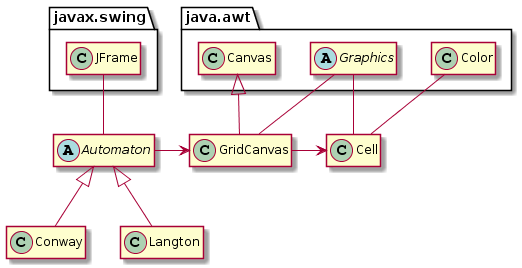
\includegraphics[width=0.75\textwidth]{figs/uml2.png}
\caption{UML class diagram of \java{Conway} and \java{Langton} applications.}
\label{fig:uml2}
\end{center}
\end{figure}

\index{IS-A}
\index{HAS-A}

The diagram shows three examples of inheritance: \java{Conway} is an \java{Automaton}, \java{Langton} is an \java{Automaton}, and \java{GridCanvas} is a Canvas.
It also shows two examples of composition: \java{Automaton} has a \java{GridCanvas}, and \java{GridCanvas} has a 2D array of \java{Cell}s.

The diagram also shows that \java{Automaton} uses \java{JFrame}, \java{GridCanvas} uses \java{Graphics}, and \java{Cell} uses \java{Graphics} and \java{Color}.

\java{Automaton} is in italics to indicate that it is an abstract class.
As it happens, \java{Graphics} is an abstract class, too.

%According to the documentation, its design ``allows an application to draw onto components that are realized on various devices, as well as onto off-screen images.''
%That's the beauty of abstraction; our code works regardless how and where it's drawn.

One of the challenges of object-oriented programming is keeping track of a large number of classes and the relationships between them.
UML class diagrams can help.


\section{Vocabulary}

\begin{description}

\term{refactor}
The process of restructuring or reorganizing existing code without changing its behavior.

\term{abstract class}
A class that is declared as \java{abstract}; it cannot be instantiated, and it may (or may not) include abstract methods.

\term{concrete class}
A class that is {\em not} declared as \java{abstract}; each of its methods must have an implementation.

\end{description}


\section{Exercises}

The code for this chapter is in the {\it ch16} directory of {\it ThinkJavaCode2}.
See page~\pageref{code} for instructions on how to download the repository.
Before you start the exercises, we recommend that you compile and run the examples.

\begin{exercise}

The last section of this chapter introduced \java{Automaton} as an abstract class and rewrote \java{Conway} as a subclass of \java{Automaton}.
Now it's your turn: rewrite \java{Langton} as a subclass of \java{Automaton}, removing the code that's no longer needed.

\end{exercise}


\begin{exercise}

Mathematically speaking, Game of Life and Langton's Ant are cellular automata, where ``cellular'' means it has cells, and ``automaton'' means it runs itself.
See \url{https://en.wikipedia.org/wiki/Cellular_automaton} for more discussion.

Implement another cellular automaton of your choice.
You may have to modify \java{Cell} and/or \java{GridCanvas}, in addition to extending \java{Automaton}.
For example, Brian's Brain (\url{https://en.wikipedia.org/wiki/Brian's_Brain}) requires three states: ``on'', ``dying'', and ``off''.

\end{exercise}


\end{document}
